\documentclass[10pt,a4paper,landscape]{article}

\usepackage[utf8]{inputenc}
\usepackage[T1]{fontenc}
\usepackage[french]{babel}

\usepackage{styles/couleurs}
\usepackage{styles/boites}
\usepackage{styles/maths}
\usepackage{styles/figures}

\usepackage{amsmath}
\usepackage{amssymb}
\usepackage{graphicx}
\usepackage[most]{tcolorbox}
\usepackage{geometry}

\geometry{
  a4paper,
  landscape,
  left=7mm,
  right=7mm,
  top=7mm,
  bottom=7mm
}

\pagestyle{empty}
\setlength{\parindent}{0pt}
\setlength{\parskip}{0pt}

\begin{document}

\noindent

% =========================================================
% ACTIVITÉ DE GAUCHE
% =========================================================

\begin{minipage}[t]{0.48\textwidth}
\vspace{0pt}

\begin{center}

{\sffamily\Large\bfseries\color{TitreC}
Séquence 2 -- Théorème de Pythagore}

\vspace{0.1em}

{\sffamily\normalsize\bfseries\color{SavoirC}
Activité 1 -- Le puzzle de Pythagore}

\end{center}

\vspace{0.3em}

\small

Les mathématiciens se sont intéressés à la famille des
\textbf{triangles rectangles}.

Voici ce qu'ils ont découvert :

\vspace{0.3em}

\begin{center}

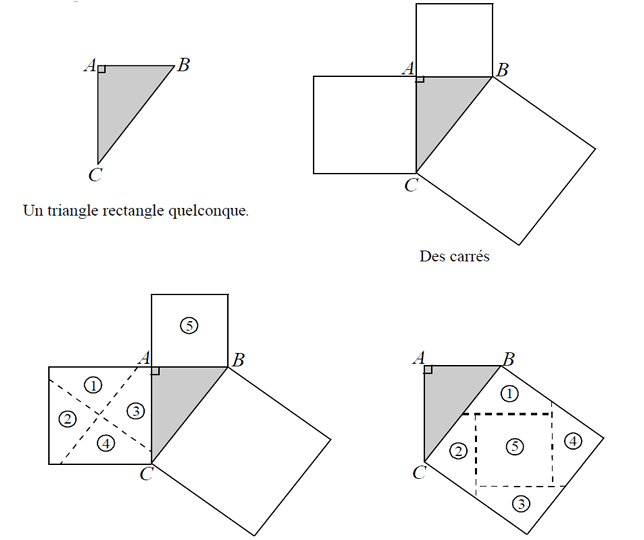
\includegraphics[
  width=0.70\linewidth,
  height=6.8cm,
  keepaspectratio
]{images/puzzle_original.png}

\end{center}

\vspace{0.2em}

\begin{tcolorbox}[
  enhanced,
  colback=SavoirBg,
  colframe=SavoirC!45,
  boxrule=0.5pt,
  arc=1.5mm,
  left=2.5mm,
  right=2.5mm,
  top=1.5mm,
  bottom=1.5mm,
  before skip=1mm,
  after skip=2mm
]

Le carré de taille intermédiaire a été partagé en
\textbf{quatre morceaux}.

Ces quatre morceaux peuvent être déplacés, sans être déformés.

Avec le petit carré, ils permettent de
\textbf{recouvrir exactement le grand carré}.

\end{tcolorbox}

\begin{tcolorbox}[
  enhanced,
  colback=ActionC!5,
  colframe=ActionC!60,
  boxrule=0.6pt,
  arc=2mm,
  left=3mm,
  right=3mm,
  top=2mm,
  bottom=2mm,
  before skip=1mm,
  after skip=0mm
]

{\sffamily\bfseries\normalsize\color{ActionC}
À vous de chercher}

\vspace{0.3em}

On considère maintenant un triangle \(ABC\) rectangle en \(A\)
tel que :

\[
AB=5\ \text{cm}
\qquad\text{et}\qquad
AC=12\ \text{cm}.
\]

\vspace{-0.3em}

\textbf{À quoi peut servir la découverte des mathématiciens
dans cette situation ?}

\smallskip

\textbf{Explique ton raisonnement.}

\end{tcolorbox}

\end{minipage}%
\hfill%
% =========================================================
% ACTIVITÉ DE DROITE
% =========================================================
\begin{minipage}[t]{0.48\textwidth}
\vspace{0pt}

\begin{center}

{\sffamily\Large\bfseries\color{TitreC}
Séquence 2 -- Théorème de Pythagore}

\vspace{0.1em}

{\sffamily\normalsize\bfseries\color{SavoirC}
Activité 1 -- Le puzzle de Pythagore}

\end{center}

\vspace{0.3em}

\small

Les mathématiciens se sont intéressés à la famille des
\textbf{triangles rectangles}.

Voici ce qu'ils ont découvert :

\vspace{0.3em}

\begin{center}

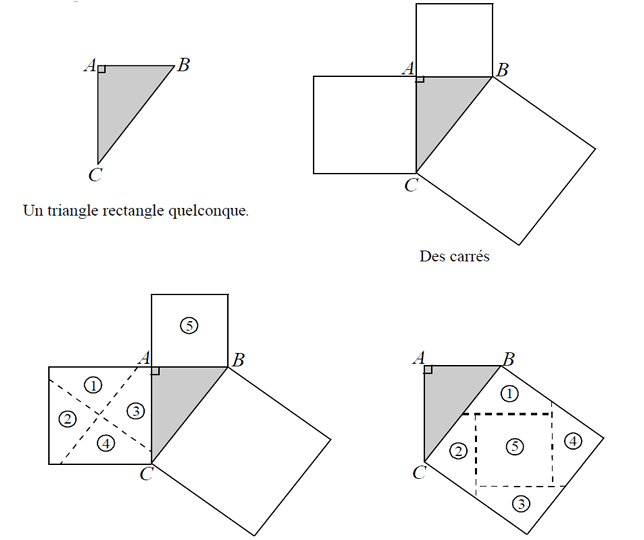
\includegraphics[
  width=0.70\linewidth,
  height=6.8cm,
  keepaspectratio
]{images/puzzle_original.png}

\end{center}

\vspace{0.2em}

\begin{tcolorbox}[
  enhanced,
  colback=SavoirBg,
  colframe=SavoirC!45,
  boxrule=0.5pt,
  arc=1.5mm,
  left=2.5mm,
  right=2.5mm,
  top=1.5mm,
  bottom=1.5mm,
  before skip=1mm,
  after skip=2mm
]

Le carré de taille intermédiaire a été partagé en
\textbf{quatre morceaux}.

Ces quatre morceaux peuvent être déplacés, sans être déformés.

Avec le petit carré, ils permettent de
\textbf{recouvrir exactement le grand carré}.

\end{tcolorbox}

\begin{tcolorbox}[
  enhanced,
  colback=ActionC!5,
  colframe=ActionC!60,
  boxrule=0.6pt,
  arc=2mm,
  left=3mm,
  right=3mm,
  top=2mm,
  bottom=2mm,
  before skip=1mm,
  after skip=0mm
]

{\sffamily\bfseries\normalsize\color{ActionC}
À vous de chercher}

\vspace{0.3em}

On considère maintenant un triangle \(ABC\) rectangle en \(A\)
tel que :

\[
AB=5\ \text{cm}
\qquad\text{et}\qquad
AC=12\ \text{cm}.
\]

\vspace{-0.3em}

\textbf{À quoi peut servir la découverte des mathématiciens
dans cette situation ?}

\smallskip

\textbf{Explique ton raisonnement.}

\end{tcolorbox}

\end{minipage}

\end{document}